% Edited version: RCX Core Engine 
% wrapper.tex -- Final wrapper for RCX Core Engine with tabularx support
\documentclass[10pt]{article}

%%% Encoding & Fonts %%%
\usepackage[utf8]{inputenc}
\usepackage{tikz}
\usetikzlibrary{positioning}
\usepackage[T1]{fontenc}
\usepackage{lmodern}
\usepackage{microtype}

%%% Spacing & Wrapping %%%
\usepackage{setspace}
\onehalfspacing
\sloppy
\emergencystretch=3em

%%% Page Layout %%%
\usepackage{geometry}
\geometry{margin=1in}

%%% Table Wrapping %%%
\usepackage{tabularx}

%%% Math Breaks %%%
\binoppenalty=1000
\relpenalty=1000

%%% Mathematics & Lists %%%
\usepackage{amsmath,amssymb}
\allowdisplaybreaks
\usepackage{enumitem}
\setlist{nosep,topsep=6pt}

%%% Auto-include starred sections in ToC %%%
\makeatletter
  \let\origsection\section
  \renewcommand{\section}{\@ifstar{\secstar}{\origsection}}
  \newcommand{\secstar}[1]{%
    \origsection*{#1}%
    \addcontentsline{toc}{section}{#1}%
  }
  \let\origsubsection\subsection
  \renewcommand{\subsection}{\@ifstar{\subsecstar}{\origsubsection}}
  \newcommand{\subsecstar}[1]{%
    \origsubsection*{#1}%
    \addcontentsline{toc}{subsection}{#1}%
  }
\makeatother

%%% Hyperlinks %%%
\usepackage{hyperref}
\hypersetup{
  colorlinks,
  linkcolor=blue,
  urlcolor=teal,
  citecolor=magenta
}

%%% Tables & Multi-column support %%%
\usepackage{booktabs}
\usepackage{multicol}

%%% Headers & Footers %%%
\usepackage{fancyhdr}
\pagestyle{fancy}
\fancyhf{}
\fancyhead[L]{\textsc{RCX Core Engine}}
\fancyhead[R]{\thepage}
\renewcommand{\headrulewidth}{0.4pt}

%%% RCX Engine Parameter Macros %%%
\newcommand{\EngineParams}{\mathcal{E}=(P,m,Hash,Order,Sched)}
\newcommand{\NextID}{\mathsf{NextID}(G)}
\newcommand{\ValidID}[1]{\mathsf{ValidID}(G,#1)}
\newcommand{\EvalMap}[2]{\mathsf{EvalMap}(#1,#2,G)}
\newcommand{\IdPair}[1]{\langle \Xi(#1),\,|E(#1)|\rangle}
\newcommand{\Ident}[1]{\IdPair{#1}} 
\newcommand{\Order}{\mathrm{Order}}
\newcommand{\Sched}{\mathrm{Sched}}
\newcommand{\nablaR}{\ensuremath{\nabla R}}
\newcommand{\ACflag}{\ensuremath{\mathsf{AC\!Flag}}}
\newcommand{\RuleSymDiamond}{\ensuremath{\Diamond}}
\newcommand{\RuleSymStar}{\ensuremath{\circledast}}
\DeclareMathOperator{\GlobalStall}{GlobalStall}

%%% Document Metadata %%%
\title{RCX Core Engine  Stateless Specification}
\author{Jeffrey Abrams}
\date{10 May 2025} 

\setcounter{secnumdepth}{2}

\begin{document}
\maketitle
\tableofcontents
\bigskip

\begin{center}\small
\begin{tabular}{|c|l|}
\hline
Symbolic tag & Canonical rule number \\\hline
0.5b          & Rule 0.5(b) Global-Stall Progress \\
2.2$\Diamond$ & Rule 2.2  Closure-on-Second-Demand \\
2.3$\diamond$ & Rule 2.3  ImageClosure \\
2.3$\circledast$ & Rule 2.3* PatternClosure \\
2.4$\Diamond$ & Rule 2.4  SubsetClosure (Power Set) \\
2.6$\Diamond$ & Rule 2.6  ReflectionClosure \\\hline
\end{tabular}
\end{center}

\section*{Purpose and Positioning}
RCX is not a formal theory like ZFC or a type-theoretic calculus. It is a structural engine designed to reconstruct logic, set-like behavior, and projection operators from purely recursive containment growth. Rather than assuming symbols, logic, or axioms, RCX initiates with an empty acyclic graph and progresses only via deterministic stall-driven recursion. Traditional mathematical objects (such as $\emptyset$, $\omega$, $\mathcal P(x)$, or choice functions) are not postulated; they are introduced only if recursion stalls and their presence becomes structurally unavoidable. 

The engine is capable of reproducing fragments of ZFC, CZF, or rejecting both, depending on how closure rules resolve. It is agnostic to classical logic and functions as a deterministic generator of symbolic structure under recursive pressure.

\section*{Preface}
The engine begins with an \emph{empty} graph. On the first stall the minimal \textsc{Fix} introduces the unique vertex $0$ (denoted $\varnothing$); no EmptySet axiom is assumed.

\paragraph*{FirstFix vs.\ Projection.}
The edge $\langle 0,1\rangle$ that \textsc{Fix} inserts on the very first
stall freezes the edge-constructor operator immediately (Rule 3.1).
The \emph{label} "$\varnothing$" is \emph{not} projected at that moment;
it is introduced only after a \emph{second}, independent encounter of
the same trace-token $\tau$, in accordance with
Rule 2.2$\diamond$ (closure-on-second-demand).

\section*{Reader's Guide}

This primer sketches the three pillars of RCX in plain language,
so a first-time reader can orient before diving into the rules.

\subsection*{1.  From Stalls to Growth}
\begin{enumerate}[nosep]
\item The engine starts with the \emph{empty graph} $(\{0\},\varnothing)$.
\item A \textbf{unary map} $O$ is applied; if it makes no structural
      change the run \emph{stalls}.
\item On every stall, Rule 0.6 invokes \textsc{Fix} to add \emph{exactly one}
      containment edge that keeps the graph acyclic and changes the
      identity hash~$\Xi$.
\end{enumerate}
Detailed mechanics: Rules 0.5--0.7, Appendix A.4.
(See formula \eqref{eq:stall-pred}.)

\begin{figure}[ht]
  \centering
  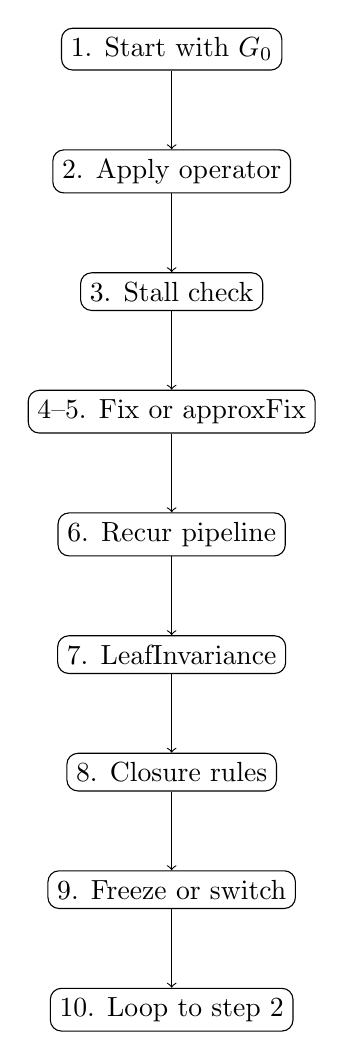
\begin{tikzpicture}[node distance=1cm, auto]
    \node[draw,rounded corners]    (start) {1. Start with $G_0$};
    \node[draw,rounded corners, below=of start]  (apply) {2. Apply operator};
    \node[draw,rounded corners, below=of apply]  (stall) {3. Stall check};
    \node[draw,rounded corners, below=of stall]  (fix)   {4--5. Fix or approxFix};
    \node[draw,rounded corners, below=of fix]    (recur) {6. Recur pipeline};
    \node[draw,rounded corners, below=of recur]  (deg)   {7. LeafInvariance};
    \node[draw,rounded corners, below=of deg]    (close) {8. Closure rules};
    \node[draw,rounded corners, below=of close]  (freeze){9. Freeze or switch};
    \node[draw,rounded corners, below=of freeze] (loop)  {10. Loop to step 2};
    \foreach \a/\b in {start/apply, apply/stall, stall/fix, fix/recur,
                      recur/deg, deg/close, close/freeze, freeze/loop}
      \draw[->] (\a) -- (\b);
  \end{tikzpicture}
  \caption{RCX engine cycle: stall-fix-promote loop.}
  \label{fig:rcx-cycle}
\end{figure}

% TODO (canonization step): add \section{00 \textbar\ RCX-$\pi$ Core Overview}

RCX-$\pi$ is a \textbf{tiny structural engine} built entirely on one primitive constructor:

\[
\mu(\;\cdot\;)
\]

Everything arises from this single form — no types, no bytecode, no opcodes.
Numbers, programs, meta-operations, and even evaluators are \emph{motifs}.
Computation occurs by \textbf{structural rewriting} rather than executing
instructions.

RCX-$\pi$ is a minimal, executable slice of RCX theory. It demonstrates how
computation can emerge from structure alone, and is deliberately small enough
that a human can inspect and evolve it directly.

%----------------------------------------------------------
\subsection{What is a Motif?}

A \textbf{motif} is a tree:

\[
\mu(\;\mu(\;\mu(\dots)\;)\;)
\]

The empty motif is:

\[
\mu()
\]

Peano naturals are nested applications of $\mu$:

\begin{center}
\begin{tabular}{c|c}
\textbf{Number} & \textbf{Motif} \\
\hline
0 & $\mu()$ \\
1 & $\mu(\mu())$ \\
2 & $\mu(\mu(\mu()))$ \\
5 & $\mu$ applied 6 times \\
\end{tabular}
\end{center}

There is no semantic type system.
A number, a closure, a tuple, a program — all are motifs.
Their identity comes only from \textbf{shape} and \textbf{reduction behavior}.

%----------------------------------------------------------
\subsection{Evaluation}

Reduction is defined in \verb|evaluator.py|.
There is no instruction set; instead RCX-$\pi$ computes by structural pattern
collapse.

Computation is visible and inspectable as geometry.

Example:

\[
\text{pred}(\text{succ}(0))
\]

reduces structurally — nothing is executed, only folded.

%----------------------------------------------------------
\subsection{Programs as Motifs}

Programs are not separate entities.
A closure \emph{is} a motif that expects activation.

\begin{center}
\begin{tabular}{l|l}
\textbf{Name} & \textbf{Meaning} \\
\hline
\verb|swap_xy_closure| & $(x,y) \rightarrow (y,x)$ \\
\verb|dup_x_closure| & $(x,y) \rightarrow (x,x)$ \\
\verb|rotate_xyz_closure| & $(x,y,z) \rightarrow (y,z,x)$ \\
\end{tabular}
\end{center}

Activation is structural growth:

\[
\text{closure} \;+\; \text{data} \; \Rightarrow \; \mu(\text{closure},\text{data})
\]

then reduction collapses the geometry into a result.
No VM stack — computation is origami.

%----------------------------------------------------------
\subsection{Activation Example}

During evaluation you can watch the motif twist and collapse.
Execution becomes visual rather than symbolic — instructions are replaced
by \emph{shape transformations}.

%----------------------------------------------------------
\subsection{Structural Classification Layer}

RCX-$\pi$ includes a minimal \textbf{meta-classifier} that inspects motifs and
tags them as:

\begin{center}
\begin{tabular}{l|l}
\textbf{Label} & \textbf{Meaning} \\
\hline
\verb|value| & numeric/atomic \\
\verb|program| & closure awaiting activation \\
\verb|mixed| & partial application \\
\verb|struct| & generic composite motif \\
\end{tabular}
\end{center}

Example classification:

\[
\text{pair}(2,5)
\;\Rightarrow\;
\langle \text{value} \rangle (2,5)
\]

Motifs become reflective — structure is visible to itself.

%----------------------------------------------------------
\subsection{Pairs, Triples, and Higher Arity}

Tuples require no new rules — they are just nested motifs.
Closures operate by rearranging structure:

\[
(x,y,z) \mapsto (y,z,x)
\]

Everything is \emph{fold, reorder, collapse}.

Structure \textbf{is} the computation.

%----------------------------------------------------------
\subsection{Why This Matters}

Traditional systems rely on:

\begin{itemize}
\item opcodes
\item call stacks
\item environments
\item interpreters evaluating interpreters
\end{itemize}

RCX-$\pi$ replaces all of this with:

\[
\text{Geometry} + \text{Reduction Rules} = \text{Computation}
\]

Programs are not written — they \textbf{grow}.
Evaluation is physical, spatial, inspectable.

%----------------------------------------------------------
\subsection{Higher-Level Toolkit (v1.2+)}

The engine remains minimal, but a standard library of structural patterns is
emerging:

\begin{center}
\begin{tabular}{l|p{7cm}}
\textbf{Feature} & \textbf{What it does} \\
\hline
\verb|motif_to_int| & collapse Peano motif to Python integer \\
\verb|num(n)| & lift Python integer to motif form \\
\verb|pretty(m)| & pretty-print motif as $(a,b,c)$ \\
\verb|bench()| & micro-benchmark evaluator \\
\verb|higher.py| & factorial, summation, map, tuple ops \\
\verb|self_host.py| & seed of eventual RCX self-boot process \\
\end{tabular}
\end{center}

All helpers are optional — the core depends on none.

%----------------------------------------------------------
\subsection{Pretty Printing}

Raw motifs are dense:

\[
\mu(\mu(\mu(\mu(\dots))))
\]

Pretty printing renders nested arity naturally:

\[
(2,5,7)
\]

allowing large RCX structures to be debugged with clarity.

%----------------------------------------------------------
\subsection{Higher-Order Combinators}

Functional patterns arise from shape alone:

\[
\text{map},\; \text{fold},\; \text{sum},\; \text{factorial}
\]

No mutation, no loops — recursion is pattern propagation.

%----------------------------------------------------------
\subsection{Benchmarks}

A tiny engine with tiny timing.
Motif reduction is light and fast — like a watch-spring.

%----------------------------------------------------------
\subsection{Vision Beyond the Core}

Today RCX-$\pi$ is a \textbf{self-consistent computational seed}.
Tomorrow:

\begin{itemize}
\item typed motifs
\item self-host evaluator
\item evolving closures
\item membrane/lobe growth
\item semantic fold → behavior
\item emergence instead of instruction
\end{itemize}

The core will not grow larger — the universe grows around it. ... \section{10 \textbar\ Visual Debugging, Structure Tracing, and Shape Introspection}

One of the greatest strengths of RCX-$\pi$ is that computation is not hidden
behind bytecode or control flow. Execution is literally the \emph{reshaping of
a tree}. This chapter formalizes tools for watching that geometry move.

The aim is simple:

\[
\text{computation} = \text{visible structure evolution}
\]

RCX-$\pi$ does not execute instructions; it folds motifs like origami.
A debugger therefore is not a stack tracer, but a \textbf{shape visualizer}.
We will build three progressively richer interfaces:

\begin{enumerate}
\item \textbf{step visualizer:} print reduction steps
\item \textbf{tree renderer:} pretty-print as ASCII shape
\item \textbf{graph visualizer:} export to \texttt{.dot}/Graphviz for render
\end{enumerate}

These tools make the runtime tangible, inspectable, and eventually
\emph{self-reflective}.

%----------------------------------------------------------
\subsection{Reduction Tracing}

The evaluator already reduces motifs through rewrite rules. We extend it with
hooks:

\begin{verbatim}
reduce(m, trace=True)
\end{verbatim}

If tracing is enabled, each reduction step is emitted:

\[
M_0 \Rightarrow M_1 \Rightarrow M_2 \Rightarrow \dots \Rightarrow M_n
\]

We show structural deltas only --- what changed between steps --- to avoid
noise with large expressions.

Example future REPL usage:

\begin{verbatim}
rcx> trace swap 2 5
step 0: μ(swap, μ(2,5))
step 1: μ(5,2)
final:  (5,2)
\end{verbatim}

%----------------------------------------------------------
\subsection{Tree Visualization (ASCII)}

Raw $\mu$-trees can be printed as nested motifs, but visual form makes patterns
obvious. We define a simple ASCII renderer:

\begin{verbatim}
μ
├─ μ
│  └─ μ()
└─ μ
   └─ μ μ μ()
\end{verbatim}

or collapsed tuple form when recognizable:

\[
(2,5,7)
\]

The visualizer becomes essential as we move toward recursion, libraries, and
mutation engines.

%----------------------------------------------------------
\subsection{Graph Rendering (DOT Export)}

We introduce an optional export format:

\begin{verbatim}
rcx> dot swap 2 5 > shape.dot
dot -Tpng shape.dot -o shape.png
\end{verbatim}

Nodes represent motif instances; edges represent children. Visualizing execution
trajectories over time yields \emph{shape films} --- a computational movie.

%----------------------------------------------------------
\subsection{Rewrite Path Maps}

Since RCX computation is geometric, its path through reductions is a graph:

\[
\{M_i\} \text{ with edges } M_i \to M_{i+1}
\]

We store these as directed graphs, enabling:

\begin{itemize}
\item comparison of reduction orders
\item detection of loops, stalls, divergent geometry
\item later: \emph{meta-motifs operating on traces}
\end{itemize}

The engine becomes observable in motion.

%----------------------------------------------------------
\subsection{Lobe and Membrane Visuals (Early Spec)}

Later RCX growth will require structures larger than tuples. We anticipate
\textbf{lobes} --- collections of motifs forming soft semantic clusters --- and
\textbf{membranes} that regulate activation boundaries.

Visual signatures may resemble:

\[
\text{motifs} \to \text{clusters} \to \text{fractal folds}
\]

Early tools will color nodes by classifier tag:

\[
\text{value} / \text{program} / \text{mixed} / \text{struct}
\]

Meta-growth becomes navigable instead of blind.

%----------------------------------------------------------
\subsection{Future Features}

\begin{itemize}
\item animated reduction playback
\item REPL modes: \texttt{:tree}, \texttt{:trace}, \texttt{:graph}
\item zoomable visual maps for large computations
\item mutation overlays to study emergent behavior
\item self-host inspection hooks
\end{itemize}

These tools move RCX-$\pi$ toward a self-aware computational ecology where
shape is not only execution, but \emph{experienceable}.

%----------------------------------------------------------
\subsection{Summary}

\begin{itemize}
\item RCX execution can be visualized --- we make tools to see shape change
\item Tracing reveals reduction paths, not call stacks
\item ASCII + Graphviz give structural insight at multiple scales
\item Lobe/membrane visuals prepare for emergent RCX organisms
\item Debugging becomes watching geometry dance
\end{itemize}

The next chapter designs the mutation engine: from stable logic to evolving
folds.
% after we place those files into docs/latex/src/
% Example:
% \section{00 \textbar\ RCX-$\pi$ Core Overview}

RCX-$\pi$ is a \textbf{tiny structural engine} built entirely on one primitive constructor:

\[
\mu(\;\cdot\;)
\]

Everything arises from this single form — no types, no bytecode, no opcodes.
Numbers, programs, meta-operations, and even evaluators are \emph{motifs}.
Computation occurs by \textbf{structural rewriting} rather than executing
instructions.

RCX-$\pi$ is a minimal, executable slice of RCX theory. It demonstrates how
computation can emerge from structure alone, and is deliberately small enough
that a human can inspect and evolve it directly.

%----------------------------------------------------------
\subsection{What is a Motif?}

A \textbf{motif} is a tree:

\[
\mu(\;\mu(\;\mu(\dots)\;)\;)
\]

The empty motif is:

\[
\mu()
\]

Peano naturals are nested applications of $\mu$:

\begin{center}
\begin{tabular}{c|c}
\textbf{Number} & \textbf{Motif} \\
\hline
0 & $\mu()$ \\
1 & $\mu(\mu())$ \\
2 & $\mu(\mu(\mu()))$ \\
5 & $\mu$ applied 6 times \\
\end{tabular}
\end{center}

There is no semantic type system.
A number, a closure, a tuple, a program — all are motifs.
Their identity comes only from \textbf{shape} and \textbf{reduction behavior}.

%----------------------------------------------------------
\subsection{Evaluation}

Reduction is defined in \verb|evaluator.py|.
There is no instruction set; instead RCX-$\pi$ computes by structural pattern
collapse.

Computation is visible and inspectable as geometry.

Example:

\[
\text{pred}(\text{succ}(0))
\]

reduces structurally — nothing is executed, only folded.

%----------------------------------------------------------
\subsection{Programs as Motifs}

Programs are not separate entities.
A closure \emph{is} a motif that expects activation.

\begin{center}
\begin{tabular}{l|l}
\textbf{Name} & \textbf{Meaning} \\
\hline
\verb|swap_xy_closure| & $(x,y) \rightarrow (y,x)$ \\
\verb|dup_x_closure| & $(x,y) \rightarrow (x,x)$ \\
\verb|rotate_xyz_closure| & $(x,y,z) \rightarrow (y,z,x)$ \\
\end{tabular}
\end{center}

Activation is structural growth:

\[
\text{closure} \;+\; \text{data} \; \Rightarrow \; \mu(\text{closure},\text{data})
\]

then reduction collapses the geometry into a result.
No VM stack — computation is origami.

%----------------------------------------------------------
\subsection{Activation Example}

During evaluation you can watch the motif twist and collapse.
Execution becomes visual rather than symbolic — instructions are replaced
by \emph{shape transformations}.

%----------------------------------------------------------
\subsection{Structural Classification Layer}

RCX-$\pi$ includes a minimal \textbf{meta-classifier} that inspects motifs and
tags them as:

\begin{center}
\begin{tabular}{l|l}
\textbf{Label} & \textbf{Meaning} \\
\hline
\verb|value| & numeric/atomic \\
\verb|program| & closure awaiting activation \\
\verb|mixed| & partial application \\
\verb|struct| & generic composite motif \\
\end{tabular}
\end{center}

Example classification:

\[
\text{pair}(2,5)
\;\Rightarrow\;
\langle \text{value} \rangle (2,5)
\]

Motifs become reflective — structure is visible to itself.

%----------------------------------------------------------
\subsection{Pairs, Triples, and Higher Arity}

Tuples require no new rules — they are just nested motifs.
Closures operate by rearranging structure:

\[
(x,y,z) \mapsto (y,z,x)
\]

Everything is \emph{fold, reorder, collapse}.

Structure \textbf{is} the computation.

%----------------------------------------------------------
\subsection{Why This Matters}

Traditional systems rely on:

\begin{itemize}
\item opcodes
\item call stacks
\item environments
\item interpreters evaluating interpreters
\end{itemize}

RCX-$\pi$ replaces all of this with:

\[
\text{Geometry} + \text{Reduction Rules} = \text{Computation}
\]

Programs are not written — they \textbf{grow}.
Evaluation is physical, spatial, inspectable.

%----------------------------------------------------------
\subsection{Higher-Level Toolkit (v1.2+)}

The engine remains minimal, but a standard library of structural patterns is
emerging:

\begin{center}
\begin{tabular}{l|p{7cm}}
\textbf{Feature} & \textbf{What it does} \\
\hline
\verb|motif_to_int| & collapse Peano motif to Python integer \\
\verb|num(n)| & lift Python integer to motif form \\
\verb|pretty(m)| & pretty-print motif as $(a,b,c)$ \\
\verb|bench()| & micro-benchmark evaluator \\
\verb|higher.py| & factorial, summation, map, tuple ops \\
\verb|self_host.py| & seed of eventual RCX self-boot process \\
\end{tabular}
\end{center}

All helpers are optional — the core depends on none.

%----------------------------------------------------------
\subsection{Pretty Printing}

Raw motifs are dense:

\[
\mu(\mu(\mu(\mu(\dots))))
\]

Pretty printing renders nested arity naturally:

\[
(2,5,7)
\]

allowing large RCX structures to be debugged with clarity.

%----------------------------------------------------------
\subsection{Higher-Order Combinators}

Functional patterns arise from shape alone:

\[
\text{map},\; \text{fold},\; \text{sum},\; \text{factorial}
\]

No mutation, no loops — recursion is pattern propagation.

%----------------------------------------------------------
\subsection{Benchmarks}

A tiny engine with tiny timing.
Motif reduction is light and fast — like a watch-spring.

%----------------------------------------------------------
\subsection{Vision Beyond the Core}

Today RCX-$\pi$ is a \textbf{self-consistent computational seed}.
Tomorrow:

\begin{itemize}
\item typed motifs
\item self-host evaluator
\item evolving closures
\item membrane/lobe growth
\item semantic fold → behavior
\item emergence instead of instruction
\end{itemize}

The core will not grow larger — the universe grows around it.
% \section{01 \textbar\ Getting Started}

This document is the practical entry point into RCX-$\pi$.
After reading this section you should be able to:

\begin{itemize}
    \item clone the repository and enter the working directory,
    \item run the full demo + test suite,
    \item experiment interactively using the minimal REPL,
    \item understand where to go next in the documentation.
\end{itemize}

RCX-$\pi$ is intentionally small --- you can inspect and understand the full
core in one sitting. This section gets your hands on a living instance quickly
rather than only reading abstract theory.

%----------------------------------------------------------
\subsection{1. Clone the Repository}

\begin{verbatim}
git clone https://github.com/jabramsja/rcx-pi-core.git
cd rcx-pi-core/WorkingRCX
\end{verbatim}

The working tree contains:

\begin{verbatim}
WorkingRCX/
  rcx_pi/            # Core RCX-π package
  demo_rcx_pi.py     # End-to-end demonstration
  example_numbers.py # Peano / arithmetic examples
  example_rcx.py     # Closure / swap / rotate examples
  example_higher.py  # Higher-level helpers (factorial, map/sum)
  bench_rcx.py       # Micro benchmark for reductions
  repl_rcx.py        # Minimal interactive REPL
  run_all.py         # Unified test + demo runner
  tests/             # Validation scripts
\end{verbatim}

No installation step is required --- the engine runs locally in-place.

%----------------------------------------------------------
\subsection{2. Python Environment}

A standard CPython $\geq$ 3.10 is recommended.

\begin{verbatim}
python3 --version
\end{verbatim}

On macOS and Linux the usual invocation is:

\begin{verbatim}
python3 run_all.py
\end{verbatim}

(Replace \verb|python3| with \verb|python| if your system maps it to Python~3.)

%----------------------------------------------------------
\subsection{3. Run the Full Demo \& Test Suite}

From inside \verb|WorkingRCX/|:

\begin{verbatim}
python3 run_all.py
\end{verbatim}

Expected output structure:

\begin{verbatim}
=== RCX-π Full Test & Demo Runner ===

>>> Running demo_rcx_pi.py
[OK]

>>> Running example_numbers.py
[OK]

>>> Running test_*.py
[OK]

=== End of RCX-π test suite ===
\end{verbatim}

If a failure occurs, the runner shows the failing script and a traceback.
You can execute a single component directly:

\begin{verbatim}
python3 demo_rcx_pi.py
python3 example_rcx.py
python3 tests/test_numbers.py
\end{verbatim}

%----------------------------------------------------------
\subsection{4. Interactive REPL}

Launch:

\begin{verbatim}
python3 repl_rcx.py
\end{verbatim}

You should see:

\begin{verbatim}
=== RCX-π REPL ===
Type 'help' for commands, 'quit' to exit.
rcx>
\end{verbatim}

Example session:

\paragraph{Peano Numbers}

\begin{verbatim}
rcx> num 5
motif: μ(μ(μ(μ(μ(μ())))))
int:   5
\end{verbatim}

\paragraph{Pairs \& structural programs}

\begin{verbatim}
rcx> pair 2 5
motif: μ(μ(μ(μ())), μ(μ(μ(μ(μ(μ()))))))
pair:  (2, 5)

rcx> swap 2 5
...
reduced => (5, 2)

rcx> rot 2 5 7
...
reduced => (5, 7, 2)
\end{verbatim}

\paragraph{Meta classification}

\begin{verbatim}
rcx> classify pair 2 5
motif:    μ(...)
tagged:   μ(tag, payload)
pretty:   <value> (2, 5)
\end{verbatim}

\paragraph{Safety Probes}

\begin{verbatim}
rcx> safe num 5
is_self_host_safe: True

rcx> safe pair 2 5
is_self_host_safe: True
\end{verbatim}

\verb|help| in the REPL lists available commands.

%----------------------------------------------------------
\subsection{5. Optional Shell Shortcuts}

If you frequently enter the working directory, you may define aliases.

Example for \verb|~/.zshrc|:

\begin{verbatim}
alias wrx='cd ~/Desktop/RCX_X/RCXStack/RCXStackminimal/WorkingRCX'
alias gl='git log --oneline --graph --decorate --all'
\end{verbatim}

Reload:

\begin{verbatim}
source ~/.zshrc
wrx   # jump directly to WorkingRCX/
gl    # view prettified git history
\end{verbatim}

Adjust the path in \verb|wrx| to match your environment.

%----------------------------------------------------------
\subsection{6. Where to Go Next}

Once \verb|run_all.py| passes with \verb|[OK]| and you have played inside the
REPL, move deeper:

\begin{itemize}
    \item \textbf{00-overview} --- motivation and conceptual framing
    \item \textbf{02-core-structures} --- motif representation and evaluation
    \item \textbf{03-program-library} --- structural programs and composition
\end{itemize}

You now have a live RCX-$\pi$ environment and the shortest path to experiments.
From here the system opens outward: self-hosting, growth laws, meta tags,
recursion scaffolds and the eventual RCX higher manifolds.
% ...
% \section{10 \textbar\ Visual Debugging, Structure Tracing, and Shape Introspection}

One of the greatest strengths of RCX-$\pi$ is that computation is not hidden
behind bytecode or control flow. Execution is literally the \emph{reshaping of
a tree}. This chapter formalizes tools for watching that geometry move.

The aim is simple:

\[
\text{computation} = \text{visible structure evolution}
\]

RCX-$\pi$ does not execute instructions; it folds motifs like origami.
A debugger therefore is not a stack tracer, but a \textbf{shape visualizer}.
We will build three progressively richer interfaces:

\begin{enumerate}
\item \textbf{step visualizer:} print reduction steps
\item \textbf{tree renderer:} pretty-print as ASCII shape
\item \textbf{graph visualizer:} export to \texttt{.dot}/Graphviz for render
\end{enumerate}

These tools make the runtime tangible, inspectable, and eventually
\emph{self-reflective}.

%----------------------------------------------------------
\subsection{Reduction Tracing}

The evaluator already reduces motifs through rewrite rules. We extend it with
hooks:

\begin{verbatim}
reduce(m, trace=True)
\end{verbatim}

If tracing is enabled, each reduction step is emitted:

\[
M_0 \Rightarrow M_1 \Rightarrow M_2 \Rightarrow \dots \Rightarrow M_n
\]

We show structural deltas only --- what changed between steps --- to avoid
noise with large expressions.

Example future REPL usage:

\begin{verbatim}
rcx> trace swap 2 5
step 0: μ(swap, μ(2,5))
step 1: μ(5,2)
final:  (5,2)
\end{verbatim}

%----------------------------------------------------------
\subsection{Tree Visualization (ASCII)}

Raw $\mu$-trees can be printed as nested motifs, but visual form makes patterns
obvious. We define a simple ASCII renderer:

\begin{verbatim}
μ
├─ μ
│  └─ μ()
└─ μ
   └─ μ μ μ()
\end{verbatim}

or collapsed tuple form when recognizable:

\[
(2,5,7)
\]

The visualizer becomes essential as we move toward recursion, libraries, and
mutation engines.

%----------------------------------------------------------
\subsection{Graph Rendering (DOT Export)}

We introduce an optional export format:

\begin{verbatim}
rcx> dot swap 2 5 > shape.dot
dot -Tpng shape.dot -o shape.png
\end{verbatim}

Nodes represent motif instances; edges represent children. Visualizing execution
trajectories over time yields \emph{shape films} --- a computational movie.

%----------------------------------------------------------
\subsection{Rewrite Path Maps}

Since RCX computation is geometric, its path through reductions is a graph:

\[
\{M_i\} \text{ with edges } M_i \to M_{i+1}
\]

We store these as directed graphs, enabling:

\begin{itemize}
\item comparison of reduction orders
\item detection of loops, stalls, divergent geometry
\item later: \emph{meta-motifs operating on traces}
\end{itemize}

The engine becomes observable in motion.

%----------------------------------------------------------
\subsection{Lobe and Membrane Visuals (Early Spec)}

Later RCX growth will require structures larger than tuples. We anticipate
\textbf{lobes} --- collections of motifs forming soft semantic clusters --- and
\textbf{membranes} that regulate activation boundaries.

Visual signatures may resemble:

\[
\text{motifs} \to \text{clusters} \to \text{fractal folds}
\]

Early tools will color nodes by classifier tag:

\[
\text{value} / \text{program} / \text{mixed} / \text{struct}
\]

Meta-growth becomes navigable instead of blind.

%----------------------------------------------------------
\subsection{Future Features}

\begin{itemize}
\item animated reduction playback
\item REPL modes: \texttt{:tree}, \texttt{:trace}, \texttt{:graph}
\item zoomable visual maps for large computations
\item mutation overlays to study emergent behavior
\item self-host inspection hooks
\end{itemize}

These tools move RCX-$\pi$ toward a self-aware computational ecology where
shape is not only execution, but \emph{experienceable}.

%----------------------------------------------------------
\subsection{Summary}

\begin{itemize}
\item RCX execution can be visualized --- we make tools to see shape change
\item Tracing reveals reduction paths, not call stacks
\item ASCII + Graphviz give structural insight at multiple scales
\item Lobe/membrane visuals prepare for emergent RCX organisms
\item Debugging becomes watching geometry dance
\end{itemize}

The next chapter designs the mutation engine: from stable logic to evolving
folds.

\end{document}
